% Localization benchmark in simulation: findings report.
% Build: latexmk -pdf main.tex   (figures/ and tables/ come from scripts/report_figures.py)
\documentclass[11pt,letterpaper]{article}

% ---------------------------------------------------------------- packages
\usepackage[T1]{fontenc}
\usepackage[utf8]{inputenc}
\usepackage{lmodern}
\usepackage[final]{microtype}
\usepackage[margin=1in,headheight=14pt]{geometry}
\usepackage{amsmath}
\usepackage{graphicx}
\usepackage[export]{adjustbox}
\usepackage{booktabs}
\usepackage{array}
\usepackage{makecell}
\renewcommand{\theadfont}{\normalsize}
\usepackage{tabularx}
\usepackage[detect-all]{siunitx}
\usepackage[table]{xcolor}
\usepackage{caption}
\usepackage{subcaption}
\usepackage{enumitem}
\usepackage{fancyhdr}
\usepackage{placeins}
% let floats share pages with text instead of collecting on half-empty float pages
\renewcommand{\topfraction}{0.9}
\renewcommand{\bottomfraction}{0.8}
\renewcommand{\textfraction}{0.07}
\renewcommand{\floatpagefraction}{0.75}
\setcounter{topnumber}{3}
\setcounter{bottomnumber}{2}
\setcounter{totalnumber}{5}
\makeatletter\setlength{\@fptop}{0pt}\makeatother
\usepackage{tikz}
\usetikzlibrary{arrows.meta,positioning,fit,backgrounds,calc}
\usepackage[most]{tcolorbox}
\usepackage[hidelinks]{hyperref}
\usepackage[capitalise,noabbrev]{cleveref}

% ---------------------------------------------------------------- style
\definecolor{scan}{HTML}{2A78D6}
\definecolor{amcl}{HTML}{EB6834}
\definecolor{slam}{HTML}{1BAF7A}
\definecolor{odom}{HTML}{8F8E89}
\definecolor{ink}{HTML}{1F1F1F}
\definecolor{ink2}{HTML}{5A5A5A}
\definecolor{panel}{HTML}{F4F6F9}
\definecolor{rule}{HTML}{B8C3D3}
\newcommand{\swatch}[1]{\textcolor{#1}{\rule[0.05em]{0.75em}{0.75em}}}

\captionsetup{font=small,labelfont=bf,labelsep=period,margin=0.2in}
\captionsetup[table]{position=top,skip=4pt}
\setlist{itemsep=2pt,topsep=4pt,parsep=0pt}
\setlength{\parskip}{3pt}
\renewcommand{\arraystretch}{1.12}
\sisetup{range-phrase=--,range-units=single}

\pagestyle{fancy}
\fancyhf{}
\fancyhead[L]{\small\color{ink2}Localization in simulation: findings}
\fancyhead[R]{\small\color{ink2}Ingenuity Labs Localization Team}
\fancyfoot[C]{\small\thepage}
\renewcommand{\headrulewidth}{0.4pt}

\newcommand{\code}[1]{\texttt{#1}}
\newcommand{\tablenote}[1]{\par\vspace{3pt}{\footnotesize\color{ink2}#1\par}}

% generated by scripts/report_figures.py: values quoted in the text, used as \val{key}
\makeatletter
\@namedef{val@amcl-filled-p95}{24.5}
\@namedef{val@amcl-n0-lost}{0/3}
\@namedef{val@amcl-n0-rmse}{6.2}
\@namedef{val@amcl-n0-yaw}{1.2}
\@namedef{val@amcl-n1-lost}{0/3}
\@namedef{val@amcl-n1-rmse}{9.4}
\@namedef{val@amcl-n1-yaw}{1.9}
\@namedef{val@amcl-n2-lost}{0/3}
\@namedef{val@amcl-n2-rmse}{13.4}
\@namedef{val@amcl-n2-yaw}{2.7}
\@namedef{val@amcl-n4-lost}{1/3}
\@namedef{val@amcl-n4-rmse}{23.7}
\@namedef{val@amcl-n4-yaw}{4.4}
\@namedef{val@amcl-n8-lost}{3/3}
\@namedef{val@amcl-n8-rmse}{36.5}
\@namedef{val@amcl-n8-yaw}{6.7}
\@namedef{val@amcl-outline-lost}{0/17}
\@namedef{val@amcl-outline-p95}{11.2}
\@namedef{val@amcl-outline-rmse}{6.3}
\@namedef{val@amcl-outline-yaw}{1.1}
\@namedef{val@amcl-sweep-lost}{6/17}
\@namedef{val@amcl-sweep-rmse}{12.4}
\@namedef{val@amcl-sweep-yaw}{2.6}
\@namedef{val@noise-rtf-max}{1.00}
\@namedef{val@noise-rtf-min}{0.85}
\@namedef{val@odom-n0-lost}{0/3}
\@namedef{val@odom-n0-rmse}{0.0}
\@namedef{val@odom-n0-yaw}{0.0}
\@namedef{val@odom-n1-lost}{3/3}
\@namedef{val@odom-n1-rmse}{2.2}
\@namedef{val@odom-n1-yaw}{24.5}
\@namedef{val@odom-n2-lost}{3/3}
\@namedef{val@odom-n2-rmse}{4.2}
\@namedef{val@odom-n2-yaw}{48.9}
\@namedef{val@odom-n4-lost}{3/3}
\@namedef{val@odom-n4-rmse}{6.9}
\@namedef{val@odom-n4-yaw}{97.8}
\@namedef{val@odom-n8-lost}{3/3}
\@namedef{val@odom-n8-rmse}{7.6}
\@namedef{val@odom-n8-yaw}{101}
\@namedef{val@runs-noise}{60}
\@namedef{val@scan-n0-lost}{0/3}
\@namedef{val@scan-n0-rmse}{4.0}
\@namedef{val@scan-n0-yaw}{0.5}
\@namedef{val@scan-n1-lost}{0/3}
\@namedef{val@scan-n1-rmse}{4.3}
\@namedef{val@scan-n1-yaw}{0.6}
\@namedef{val@scan-n2-lost}{0/3}
\@namedef{val@scan-n2-rmse}{4.6}
\@namedef{val@scan-n2-yaw}{0.6}
\@namedef{val@scan-n4-lost}{0/3}
\@namedef{val@scan-n4-rmse}{5.3}
\@namedef{val@scan-n4-yaw}{0.9}
\@namedef{val@scan-n8-lost}{0/3}
\@namedef{val@scan-n8-rmse}{11.6}
\@namedef{val@scan-n8-yaw}{2.6}
\@namedef{val@scan-sweep-lost}{0/17}
\@namedef{val@scan-sweep-rmse}{5.1}
\@namedef{val@scan-sweep-yaw}{0.6}
\@namedef{val@slam-fixed-lost}{0/15 (+2 failed)}
\@namedef{val@slam-fixed-p95}{8.0}
\@namedef{val@slam-fixed-rmse}{5.2}
\@namedef{val@slam-fixed-rtf-max}{0.99}
\@namedef{val@slam-fixed-rtf-min}{0.53}
\@namedef{val@slam-fixed-yaw}{0.7}
\@namedef{val@slam-lc-off-max}{8.6}
\@namedef{val@slam-lc-off-rmse}{5.0}
\@namedef{val@slam-lc-on-max}{145}
\@namedef{val@slam-lc-on-rmse}{47.0}
\@namedef{val@slam-n0-lost}{0/3}
\@namedef{val@slam-n0-rmse}{5.2}
\@namedef{val@slam-n0-yaw}{0.8}
\@namedef{val@slam-n1-lost}{0/3}
\@namedef{val@slam-n1-rmse}{5.0}
\@namedef{val@slam-n1-yaw}{0.6}
\@namedef{val@slam-n2-lost}{0/3}
\@namedef{val@slam-n2-rmse}{5.0}
\@namedef{val@slam-n2-yaw}{0.6}
\@namedef{val@slam-n4-lost}{0/3}
\@namedef{val@slam-n4-rmse}{5.3}
\@namedef{val@slam-n4-yaw}{0.8}
\@namedef{val@slam-n8-lost}{0/3}
\@namedef{val@slam-n8-rmse}{7.3}
\@namedef{val@slam-n8-yaw}{1.6}
\@namedef{val@slam-ref-off-max}{22.1}
\@namedef{val@slam-ref-off-rmse}{9.5}
\@namedef{val@slam-ref-on-max}{213}
\@namedef{val@slam-ref-on-rmse}{86.6}
\@namedef{val@slam-sweep-lost}{17/17}
\@namedef{val@slam-sweep-rmse}{92.9}
\@namedef{val@slam-sweep-yaw}{7.9}
\@namedef{val@victoria_ref-rest-within10}{93}
\@namedef{val@victoria_ref-start-within10}{74}
\@namedef{val@victoria_ref_lc-rest-within10}{86}
\@namedef{val@victoria_ref_lc-start-within10}{91}
\newcommand{\val}[1]{\@ifundefined{val@#1}{\textbf{??}}{\@nameuse{val@#1}}}
\makeatother


\title{\vspace{-1.6cm}\textbf{Localization in Simulation:\\AMCL, SLAM Toolbox and a Scan Matcher on the Victoria Track}}
\author{Ingenuity Labs Localization Team}
\date{22 November 2026\vspace{-0.4cm}}

\begin{document}
\maketitle
\thispagestyle{fancy}

\begin{abstract}
\noindent
We compared three 2D lidar localizers in a Gazebo simulation of the Victoria track: Nav2 AMCL,
SLAM Toolbox in localization mode, and a scan-to-map matcher written for this project. A speed
sweep with perfect odometry exposed a configuration problem in each of the first two: AMCL scored
lidar beams against a map whose off-track area is filled in, and SLAM Toolbox re-optimized its map
on wrong loop closures during localization. With both fixed, all three reach \SIrange{4}{6}{cm}.
Under simulated odometry error of up to eight times our real-car estimate, SLAM Toolbox was the
most robust, the scan matcher the most accurate at low noise, and AMCL degraded steadily until it
lost track.
\end{abstract}

\begin{tcolorbox}[enhanced,colback=panel,colframe=rule,boxrule=0.5pt,arc=2pt,left=8pt,right=8pt,
                  top=6pt,bottom=6pt,title={\bfseries Summary of findings},coltitle=ink,
                  colbacktitle=rule!45,fonttitle=\normalsize]
\begin{itemize}[leftmargin=1.2em]
  \item \textbf{No speed dependence} between 0.20 and \SI{1.00}{m/s} for any localizer: failures
        are tied to places on the track and to configuration, not to speed.
  \item \textbf{AMCL needs a walls-only map.} On the filled map: \SI{\val{amcl-sweep-rmse}}{cm},
        lost track in \val{amcl-sweep-lost} runs. On the outline map: \SI{\val{amcl-outline-rmse}}{cm},
        \val{amcl-outline-lost}.
  \item \textbf{SLAM Toolbox needs loop closure off in localization mode.} With it on, wrong
        matches re-optimize the whole graph and move the map; it lost track in every run. With it
        off: \SI{\val{slam-fixed-rmse}}{cm}, no run lost.
  \item \textbf{With perfect odometry all three are within \SIrange{4}{6}{cm}}, so the speed sweep
        only shows how much a localizer disturbs good odometry.
  \item \textbf{Under odometry noise SLAM Toolbox is the most robust}, the scan matcher is the most
        accurate at low noise and falls behind only at the highest level, and AMCL's error grows with
        the noise until it loses track.
\end{itemize}
\vspace{2pt}
\centering\small
\begin{tabular}{lrrrrrr}
\toprule
 & \multicolumn{2}{c}{Perfect odometry${}^{a}$} & \multicolumn{2}{c}{Noise level 4} & \multicolumn{2}{c}{Noise level 8} \\
\cmidrule(lr){2-3}\cmidrule(lr){4-5}\cmidrule(lr){6-7}
Localizer & RMSE [cm] & Lost & RMSE [cm] & Lost & RMSE [cm] & Lost \\
\midrule
Scan matcher & 5.1 & 0/17 & 5.3 & 0/3 & 11.6 & 0/3 \\
AMCL & 6.3 & 0/17 & 23.7 & 1/3 & 36.5 & 3/3 \\
SLAM Toolbox & 5.2 & 0/15 (+2 failed) & 5.3 & 0/3 & 7.3 & 0/3 \\
\bottomrule
\end{tabular}

\tablenote{RMSE: median over runs of the position RMSE over the driving window. Lost: runs whose
error ever exceeded \SI{0.5}{m}. ${}^{a}$Speed sweep after the fixes, 17 speeds (scan matcher on
the filled map). Noise levels: 3 runs each at \SI{1.0}{m/s}, all localizers on their final maps.}
\end{tcolorbox}

% =====================================================================
\section{Introduction}

Before a localizer runs on the car it should be understood in a setting where the true pose is
known exactly. This report summarizes a series of benchmarks run in a standalone Gazebo
simulation of the Victoria track (the \code{slam\_toolbox\_sandbox} package of our race stack). It
started as a check of whether SLAM Toolbox~\cite{macenski2021slam} could replace Cartographer and
grew into a comparison of three localizers under identical conditions:
\begin{itemize}[leftmargin=1.5em]
  \item \swatch{amcl}~\textbf{Nav2 AMCL}~\cite{macenski2020marathon}, an adaptive particle
        filter~\cite{thrun2005probabilistic,fox2003kld} on a fixed map image;
  \item \swatch{slam}~\textbf{SLAM Toolbox} in localization mode, on a pose graph it recorded itself;
  \item \swatch{scan}~\textbf{Scan matcher} (\code{scan\_match\_localizer}), a Gauss--Newton
        scan-to-map matcher on a fixed map, written for this project.
\end{itemize}
\Cref{sec:setup} describes the simulation, the localizers and how the error is measured.
\Cref{sec:sweep} presents the speed sweep and what it revealed, \cref{sec:amcl,sec:slam} the
diagnosis and fix of AMCL and SLAM Toolbox, \cref{sec:compare} the comparison after the fixes, and
\cref{sec:noise} the odometry noise test. \Cref{sec:conclusions} summarizes.

% =====================================================================
\section{Setup and methods}\label{sec:setup}

\subsection{Simulation}

\begin{figure}[htbp]
  \centering
  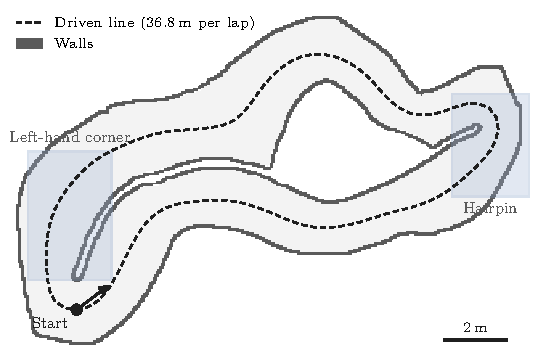
\includegraphics[max width=\linewidth]{figures/track.pdf}
  \caption{The simulated Victoria track. The walls are generated from the race stack's occupancy
  map; the autopilot drives the dashed line counter-clockwise from the start. The two shaded
  corners recur throughout the report: the hairpin, where the original AMCL lost track, and the
  left-hand corner.}
  \label{fig:track}
\end{figure}

The world is generated from the race stack's Victoria occupancy map
(\code{stack\_master/\allowbreak maps/\allowbreak Victoria}): a \SI{0.4}{m} high wall box is placed wherever an occupied
pixel touches free space, so the Gazebo frame equals the map frame (\cref{fig:track}). The car is a
differential-drive model with a lidar similar to a Hokuyo UST-10LX (\ang{270}, 1081 beams,
\SI{40}{Hz}, \SIrange{0.06}{30}{m}, Gaussian range noise $\sigma=\SI{1}{cm}$), mounted
\SI{0.1}{m} ahead of the base. Odometry is Gazebo's exact pose at \SI{50}{Hz} unless the odometry
noise of \cref{sec:noise} is switched on; ground truth is published separately and always exact.
An autopilot (pure pursuit on the centerline, \SI{36.8}{m} per lap) steers on ground truth, so
every localizer sees the same drive regardless of its estimate.

\subsection{The three localizers}

\begin{table}[htbp]
  \centering\small
  \caption{The three localizers and their configuration in the final benchmarks.}
  \label{tab:localizers}
  \begin{tabularx}{\linewidth}{@{}>{\raggedright\arraybackslash}p{2.2cm}>{\raggedright\arraybackslash}X
                                >{\raggedright\arraybackslash}X>{\raggedright\arraybackslash}X@{}}
    \toprule
    & \swatch{scan}~Scan matcher & \swatch{amcl}~AMCL (Nav2) & \swatch{slam}~SLAM Toolbox 2.6 \\
    \midrule
    Map & Fixed image, walls only (\code{victoria\_outline}) & Fixed image, walls only
        (\code{victoria\_outline}) & Own pose graph (\code{victoria\_ref\_lc}) \\
    Method & Per scan: odometry prediction, then Gauss--Newton fit of every 4th beam to a distance
        field of the walls, weak odometry prior & Particle filter, 500--2000 particles (KLD),
        likelihood-field model, 60 beams per update & Matches each scan against its last 3 scans
        and nearby map scans (Karto), weighted mean \\
    Updates & Every scan (\SI{40}{Hz}) & After \SI{0.1}{m} or \SI{0.1}{rad} & After \SI{0.1}{m} or
        \SI{0.1}{rad} \\
    Safeguards & Reject if $<30\%$ of points within \SI{0.1}{m} of a wall or correction
        $>\SI{0.5}{m}$ & Recovery off (no random particles) & Loop closure off; search window
        \SI{\pm0.25}{m} \\
    Recovers when lost & No (searches \SI{\pm0.5}{m}) & No & No \\
    \bottomrule
  \end{tabularx}
\end{table}

\Cref{tab:localizers} summarizes the localizers. AMCL and the scan matcher localize on a fixed map
image and never change it. SLAM Toolbox cannot load a plain image; it localizes on a serialized pose
graph recorded in the simulation. All three start from the true spawn pose and publish the
\code{map}$\to$\code{odom} transform.

The maps are idealized, which should be kept in mind when reading absolute numbers. AMCL and the
scan matcher get exactly the wall pixels the simulated walls were built from. SLAM Toolbox's map was
recorded with a deliberately constrained matcher (scans may move only about \SI{1}{cm} and
\ang{0.2} from the perfect odometry), which is only possible in simulation. Both are therefore
upper bounds for what the localizers would achieve on maps from a real mapping run.

\subsection{Benchmark pipeline}

\begin{figure}[htbp]
  \centering
  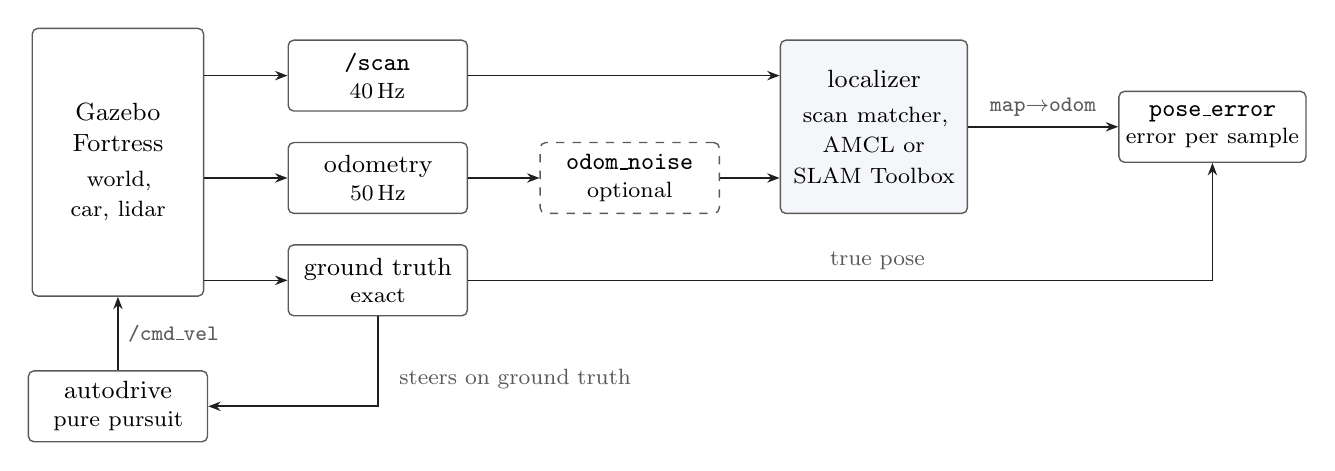
\begin{tikzpicture}[x=1mm, y=1mm, font=\small,
      box/.style={draw=ink2, line width=0.5pt, rounded corners=2pt, align=center, fill=white,
                  minimum height=9mm, inner sep=2.5pt, text width=#1},
      box/.default=21mm,
      flow/.style={-{Stealth[length=4.5pt]}, line width=0.6pt, draw=ink},
      lab/.style={font=\footnotesize, color=ink2, align=center}]
    \node[box=20mm, minimum height=34mm] (gz) at (0, 0) {Gazebo\\Fortress\\[3pt]{\footnotesize world,\\car, lidar}};
    \node[box] (scan) at (33, 11) {\code{/scan}\\[-1pt]{\footnotesize \SI{40}{Hz}}};
    \node[box] (odom) at (33, -2) {odometry\\[-1pt]{\footnotesize \SI{50}{Hz}}};
    \node[box] (gt) at (33, -15) {ground truth\\[-1pt]{\footnotesize exact}};
    \node[box=21mm, dashed] (noise) at (65, -2) {\code{odom\_noise}\\[-1pt]{\footnotesize optional}};
    \node[box=22mm, minimum height=22mm, fill=panel] (loc) at (96, 4.5)
         {localizer\\[3pt]{\footnotesize scan matcher,\\AMCL or SLAM Toolbox}};
    \node[box=22mm] (err) at (139, 4.5) {\code{pose\_error}\\[-1pt]{\footnotesize error per sample}};
    \node[box] (auto) at (0, -31) {autodrive\\[-1pt]{\footnotesize pure pursuit}};
    \draw[flow] (gz.east |- scan) -- (scan);
    \draw[flow] (gz.east |- odom) -- (odom);
    \draw[flow] (gz.east |- gt) -- (gt);
    \draw[flow] (scan) -- (loc.west |- scan);
    \draw[flow] (odom) -- (noise);
    \draw[flow] (noise) -- (loc.west |- noise);
    \draw[flow] (loc) -- node[lab, above] {\code{map}$\to$\code{odom}} (err);
    \draw[flow] (gt) -- node[lab, above, pos=0.55] {true pose} (err.south |- gt) -- (err.south);
    \draw[flow] (gt.south) |- (auto.east);
    \node[lab, anchor=west] at ($(gt.south)+(1.5,-8)$) {steers on ground truth};
    \draw[flow] (auto) -- node[lab, right] {\code{/cmd\_vel}} (gz);
  \end{tikzpicture}
  \caption{Benchmark pipeline. Each run starts a fresh simulation and one localizer; the error node
  compares the localizer's estimate \code{map}$\to$\code{base\_link} with ground truth at the same
  timestamp. In the noise test, a node between Gazebo and the localizers corrupts the odometry.}
  \label{fig:pipeline}
\end{figure}

A benchmark script runs each test case in a fresh simulation (\cref{fig:pipeline}): it starts
Gazebo, the localizer and the error node, drives the requested laps and appends one row of metrics
to a results file. Each run uses its own Gazebo partition and ROS domain, so several runs execute in
parallel without seeing each other's topics; a sweep script splits the runs over parallel workers,
longest first. Failed starts are retried up to three times and recorded if they never succeed.

\subsection{Metrics}

The error node compares, for every ground-truth message, the true pose with the localizer's estimate
at exactly the same timestamp (an older estimate would add artificial error while the car moves).
Samples whose estimate has not arrived within \SI{0.5}{s} of simulation time are skipped; in the
noise test every sample was evaluated.\footnote{The speed sweeps used an earlier version that skipped late
samples at once (median coverage 72\,\%). At \SI{1.0}{m/s} with the same configuration both versions
give the same results (AMCL 6.0 vs.\ \SI{6.2}{cm}, SLAM Toolbox 5.2 vs.\ \SI{5.2}{cm}).} All metrics cover
only the \emph{driving window}, from the car's first to its last movement, because every run also
logs the car parked for some seconds, a share that would otherwise depend on speed.
\begin{itemize}[leftmargin=1.5em]
  \item \textbf{Position RMSE}: root-mean-square position error over the run, the typical error.
  \item \textbf{p95}: the 95th percentile of the position error, the bad moments without a single
        spike deciding.
  \item \textbf{Heading RMSE}: root-mean-square heading error.
  \item \textbf{Lost track}: the position error exceeded \SI{0.5}{m} at some point (about a third of
        the track width).
  \item \textbf{Lap 1$\to$3}: RMSE of the last lap minus RMSE of the first; positive means the error
        grows.
  \item \textbf{Real-time factor}: simulated time over wall time. Below 1 the localizer gets more
        computer time per simulated second than it would on the car; runs below 0.9 are flagged.
\end{itemize}
Where a table reports several runs, the cell is the median over runs.

% =====================================================================
\section{Speed sweep}\label{sec:sweep}

\subsection{Design and rationale}

Earlier comparisons used only two speeds and single laps, and their results varied strongly from
run to run. The speed sweep was designed to answer three questions at once: does a localizer's
error depend on speed, \emph{where} on the track do failures happen, and does the error grow from
lap to lap? \Cref{tab:sweep-design} lists the test matrix.

\begin{table}[htbp]
  \centering\small
  \caption{Speed-sweep test matrix.}
  \label{tab:sweep-design}
  \begin{tabular}{@{}ll@{}}
    \toprule
    Parameter & Value \\
    \midrule
    Localizers & scan matcher, AMCL, SLAM Toolbox (configurations of the time) \\
    Speeds & 17, from 0.20 to \SI{1.00}{m/s} in steps of \SI{0.05}{m/s} \\
    Laps per run & 3, driven back to back (\SI{110}{m}) \\
    Runs per speed & 1 per localizer, each in a fresh simulation (51 runs) \\
    Odometry & perfect; start pose correct \\
    Execution & 3 parallel workers, runs balanced by expected duration (\SI{82}{min}) \\
    \bottomrule
  \end{tabular}
\end{table}

Two choices shaped the design. First, \emph{one run at each of many speeds} instead of repeated runs
at a few: if a localizer has no speed dependence, neighbouring speeds act as repeats, and if it
has one, the trend becomes visible; either way the 17 points say more than three repeats at two
speeds. Second, \emph{three laps per run}: the same place on the track is passed three times, which
separates errors tied to a location from random ones and shows whether a localizer recovers after
a bad patch. Odometry was kept perfect so that only the localizer varies between runs.

\subsection{Results}

\begin{figure}[htbp]
  \centering
  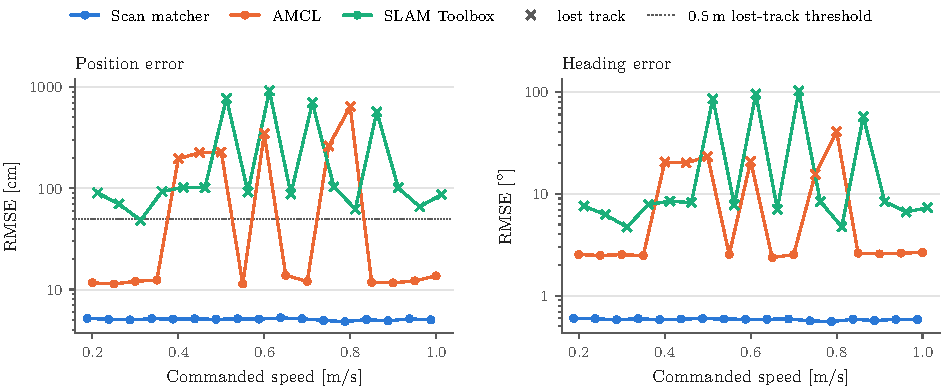
\includegraphics[max width=\linewidth]{figures/speed_sweep.pdf}
  \caption{Original speed sweep: position and heading RMSE of every run over commanded speed (log
  scales). Crosses mark runs that lost track. The scan matcher is flat at about \SI{5}{cm}; AMCL
  alternates between about \SI{12}{cm} and runs that lose track; SLAM Toolbox loses track at every
  speed.}
  \label{fig:sweep}
\end{figure}

\begin{table}[htbp]
  \centering\small
  \caption{Original speed sweep, medians over the 17 runs of each localizer.}
  \label{tab:sweep}
  \begin{tabular}{llrrrr}
\toprule
\makecell[lb]{{Localizer}} & \makecell[lb]{{Map /} \\ {configuration}} & \makecell[rb]{{RMSE} \\ {[cm]}} & \makecell[rb]{{p95} \\ {[cm]}} & \makecell[rb]{{Heading} \\ {RMSE [$^\circ$]}} & \makecell[rb]{{Lost} \\ {track}} \\
\midrule
Scan matcher & filled \texttt{Victoria.yaml} & 5.1 & 13.9 & 0.6 & 0/17 \\
AMCL & filled \texttt{Victoria.yaml} & 12.4 & 24.5 & 2.6 & 6/17 \\
SLAM Toolbox & \texttt{victoria\_ref}, loop closure on & 92.9 & 180 & 7.9 & 17/17 \\
\bottomrule
\end{tabular}

\end{table}

\Cref{fig:sweep,tab:sweep} show the results. The scan matcher was accurate and consistent:
\SI{\val{scan-sweep-rmse}}{cm} median RMSE and \ang{\val{scan-sweep-yaw}} heading error at every
speed, never lost. AMCL reached about \SI{12}{cm} in its good runs but lost track in
\val{amcl-sweep-lost} runs, with no pattern over speed. SLAM Toolbox lost track in all
\val{slam-sweep-lost} runs, with a median RMSE of \SI{\val{slam-sweep-rmse}}{cm}.

\begin{figure}[htbp]
  \centering
  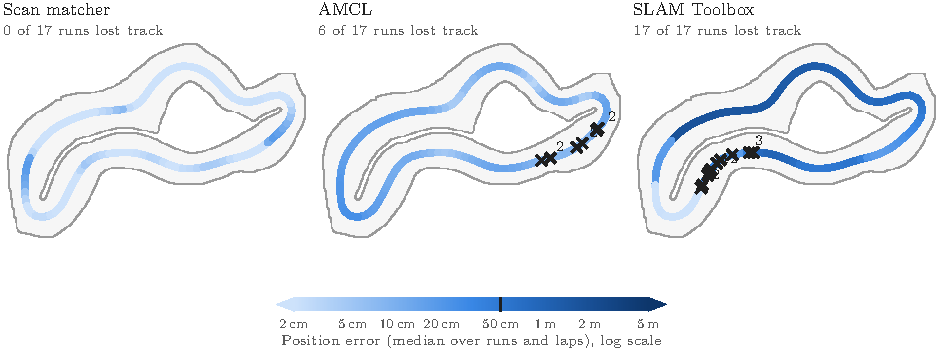
\includegraphics[max width=\linewidth]{figures/speed_sweep_track.pdf}
  \caption{Where on the track the original configurations failed. The line colour is the median
  position error at each point of the lap over all runs and laps; crosses mark where a run first
  exceeded \SI{0.5}{m} (numbers: runs in that cluster). AMCL's failures all start on the way into
  the hairpin, SLAM Toolbox's all within a few metres after the start.}
  \label{fig:sweep-track}
\end{figure}

\begin{figure}[htbp]
  \centering
  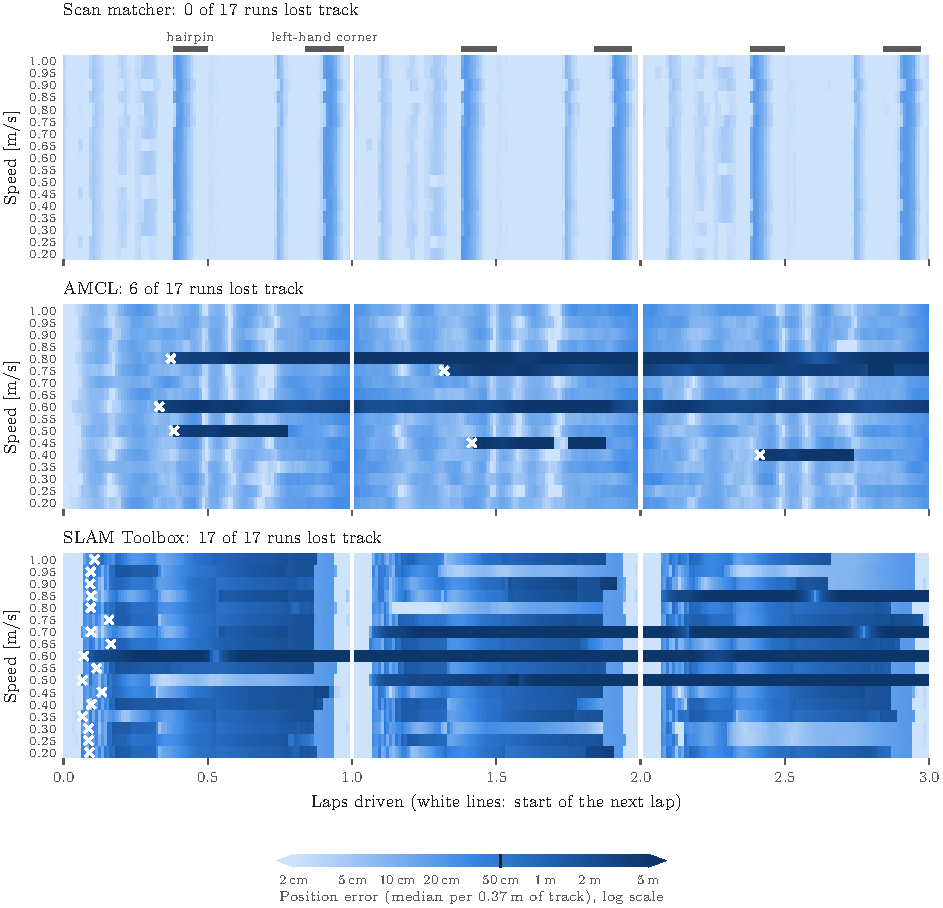
\includegraphics[max width=\linewidth]{figures/speed_sweep_heatmap.pdf}
  \caption{Error along the three laps, one row per run (speed), one cell per \SI{0.37}{m} of track.
  Columns at the same lap position are the same place on the track. The scan matcher's error rises
  slightly in the same two corners every lap. AMCL's lost runs jump to a wrong pose and stay there
  (three of them snap back after 23--35\,s). SLAM Toolbox fails about \SI{2.5}{m} after the start in
  every run and partly recovers near the start line on each lap.}
  \label{fig:sweep-heatmap}
\end{figure}

The location of the failures was the most informative result (\cref{fig:sweep-track,fig:sweep-heatmap}).
All six AMCL failures began on the stretch into the hairpin, and each was a sudden jump of
2.7--4.3\,m rather than a slow drift; three runs later snapped back, three never did. Every SLAM Toolbox run
failed at the same place, 2.5--3.5\,m after the start, and its error dropped again each time the
car passed the start line, as if its map were distorted away from the start. The scan matcher's
small error rose in the same two corners on every lap, a property of the track geometry rather
than of speed.

\paragraph{What the speed sweep taught us.}
\begin{itemize}[leftmargin=1.5em]
  \item None of the localizers depends on speed in this range; the failures are tied to locations
        and configurations, which pointed the diagnosis at the maps
        (\cref{sec:amcl,sec:slam}).
  \item The error does not grow from lap to lap for the scan matcher (lap 1$\to$3 change
        \SI{-0.1}{cm}), so with perfect odometry nothing accumulates.
  \item With perfect odometry and a correct start, a localizer that did nothing would score about
        zero. The sweep therefore measures how much a localizer \emph{disturbs} good odometry, not
        how well it \emph{corrects} bad odometry, which motivated the noise test of \cref{sec:noise}.
\end{itemize}

% =====================================================================
\FloatBarrier
\section{Fixing AMCL: the map}\label{sec:amcl}

\subsection{Diagnosis}

Nav2 AMCL weights each particle with a likelihood-field model: every beam endpoint is looked up in
a precomputed field of the distance $d$ to the nearest occupied map cell, and contributes
$p_\mathrm{hit}=\exp(-d^2/2\sigma^2)$ (with $\sigma=\SI{0.2}{m}$, plus a uniform random term).
The race stack's Victoria map, which AMCL used, is \emph{filled}: the whole area outside the track is
occupied (black), 67\,\% of all pixels. In that area $d=0$ everywhere, so a beam that passes a
wall and ends behind it scores as a perfect hit (\cref{fig:amcl-maps}a). A particle that is shifted
outwards therefore loses almost nothing, and the filter's weights become flat in exactly the
direction in which the car can be wrong.

\begin{figure}[htbp]
  \centering
  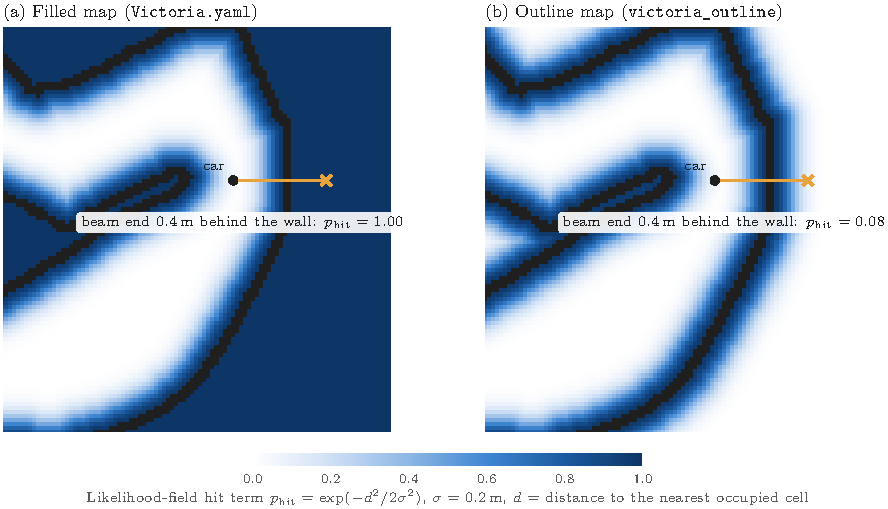
\includegraphics[max width=\linewidth]{figures/amcl_maps.pdf}
  \caption{AMCL's likelihood-field hit term in the hairpin. (a)~On the filled map every cell outside
  the track is occupied, so a beam that ends \SI{0.4}{m} behind the wall still scores
  $p_\mathrm{hit}=1$. (b)~On the outline map only the walls are occupied and the same beam scores
  close to zero, as it should. Inside the track the two fields are identical.}
  \label{fig:amcl-maps}
\end{figure}

The runs that lost track show this mechanism (\cref{fig:amcl-lost}). The estimate jumps by several
metres within a second, then follows a shifted copy of the true path, with long stretches in the
black area where the car cannot physically be. No outside reset and no warning from AMCL preceded
the jumps. With recovery disabled (no random particles are injected), the filter can only return if
particles near the truth happened to survive.

\begin{figure}[htbp]
  \centering
  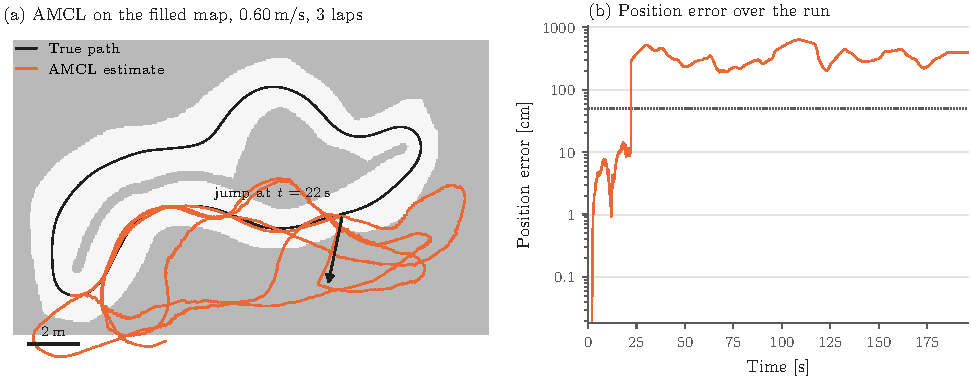
\includegraphics[max width=\linewidth]{figures/amcl_lost_run.pdf}
  \caption{A run that lost track: AMCL on the filled map at \SI{0.60}{m/s}. (a)~True path and AMCL
  estimate over three laps; grey is the occupied (filled) part of the map. After the jump the
  estimate runs parallel to the truth, largely inside the occupied area. (b)~Position error over
  time: a few centimetres, then a jump above \SI{0.5}{m} that never recovers.}
  \label{fig:amcl-lost}
\end{figure}

\subsection{Fix: an outline map}

The lidar only ever sees wall faces, so the localizer only needs the walls. A small tool
(\code{outline\_map}) keeps the occupied pixels that touch free space, using the same rule and
thickness as the world generator, so the walls are exactly the pixels the simulated walls were
built from, and marks the rest of the off-track area as unknown. Of \num{54384} occupied pixels,
\num{3829} remain. The resulting \code{victoria\_outline} map became the default for AMCL and the
scan matcher.

\subsection{Results}

\begin{figure}[htbp]
  \centering
  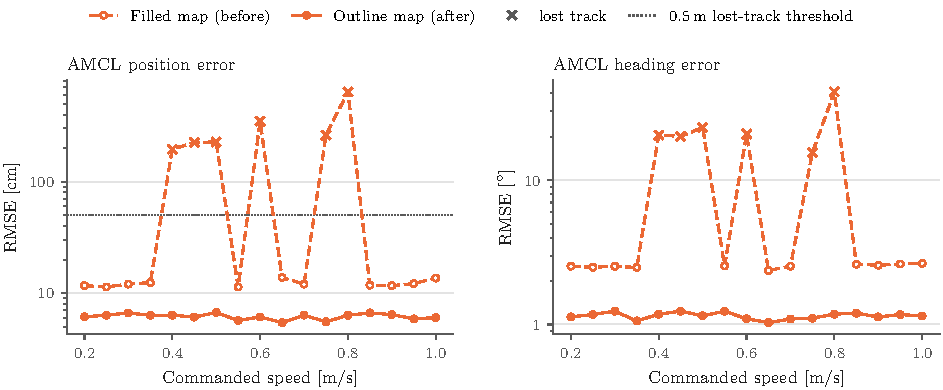
\includegraphics[max width=\linewidth]{figures/amcl_before_after.pdf}
  \caption{AMCL over speed on the filled map (before, dashed) and on the outline map (after,
  solid). On the outline map no run lost track and both errors halved, flat over speed.}
  \label{fig:amcl-ba}
\end{figure}

\begin{table}[htbp]
  \centering\small
  \caption{AMCL before and after the map change (17 runs each, 3 laps, 0.20--\SI{1.00}{m/s}).}
  \label{tab:amcl}
  \begin{tabular}{lrrrrr}
\toprule
Map & \makecell[rb]{{RMSE} \\ {[cm]}} & \makecell[rb]{{p95} \\ {[cm]}} & \makecell[rb]{{Worst run} \\ {[m]}} & \makecell[rb]{{Heading} \\ {RMSE [$^\circ$]}} & \makecell[rb]{{Lost} \\ {track}} \\
\midrule
Filled (\texttt{Victoria.yaml}) & 12.4 & 24.5 & 15.2 & 2.6 & 6/17 \\
Outline (\texttt{victoria\_outline}) & 6.3 & 11.2 & 0.2 & 1.1 & 0/17 \\
\bottomrule
\end{tabular}

  \tablenote{Worst run: the largest position error of any run.}
\end{table}

The AMCL sweep was repeated on the outline map with the same 17 speeds (\cref{fig:amcl-ba,tab:amcl}).
No run lost track (\val{amcl-outline-lost}, before \val{amcl-sweep-lost}); the median RMSE fell from
\SI{\val{amcl-sweep-rmse}}{cm} to \SI{\val{amcl-outline-rmse}}{cm}, the p95 from
\SI{\val{amcl-filled-p95}}{cm} to \SI{\val{amcl-outline-p95}}{cm}, and the heading error from
\ang{\val{amcl-sweep-yaw}} to \ang{\val{amcl-outline-yaw}}. The improvement in the runs that never
lost track shows that the filled map also flattened the weights in normal operation, not only at the
hairpin.

% =====================================================================
\FloatBarrier
\section{Fixing SLAM Toolbox: loop closure in localization mode}\label{sec:slam}

\subsection{Symptoms and a first hypothesis}

Every SLAM Toolbox run failed at the same place shortly after the start: the error was 1--2\,cm
before that point, then the estimate flipped between a few centimetres and more than half a metre
off, with heading errors of \ang{5}--\ang{16}, rather than drifting. The error dropped whenever the
car passed the start line again. A distorted map near the start explained this well.
Comparing the reference map \code{victoria\_ref} with the true walls confirmed doubled walls offset
by 10--15\,cm in the start area (\cref{fig:slam-maps}a): only \val{victoria_ref-start-within10}\,\%
of its wall pixels there lie within \SI{10}{cm} of a true wall, against
\val{victoria_ref-rest-within10}\,\% elsewhere. The map had been recorded with loop closure off, so
the drift accumulated over the mapping lap (\SI{28}{cm} and \ang{2.5} even with the constrained
matcher) remained where the lap ended, at the start.

\begin{figure}[htbp]
  \centering
  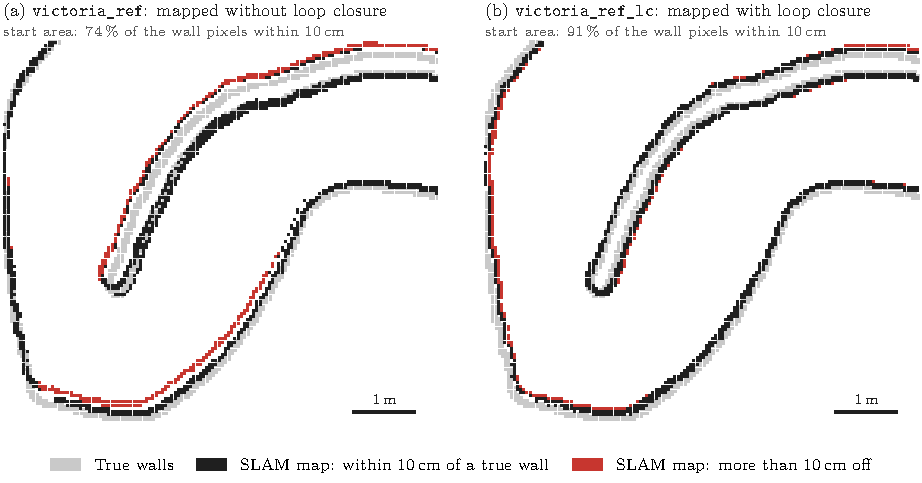
\includegraphics[max width=\linewidth]{figures/slam_maps.pdf}
  \caption{SLAM Toolbox maps in the start area against the true walls. (a)~The original reference
  map, recorded without loop closure: the end of the mapping lap left doubled, offset walls.
  (b)~Re-recorded with loop closure: the walls coincide with the true ones.}
  \label{fig:slam-maps}
\end{figure}

The map was re-recorded with loop closure on (\code{victoria\_ref\_lc}). Loop closure snapped the
\SI{28}{cm} end-of-lap error back to about \SI{3}{cm} and removed the doubled walls
(\val{victoria_ref_lc-start-within10}\,\% within \SI{10}{cm} in the start area, \cref{fig:slam-maps}b;
the correction spreads some error elsewhere, \val{victoria_ref_lc-rest-within10}\,\%). But
localization on the new map \emph{still failed at the same place}, with \SI{\val{slam-lc-on-rmse}}{cm}
RMSE and a worst error of \SI{\val{slam-lc-on-max}}{cm}. The doubled walls made things worse, but
they were not the main cause.

\subsection{Root cause}

In localization mode, SLAM Toolbox (Karto) still runs its full graph machinery on each new scan: it
matches the scan against a short rolling buffer of its own recent scans and against map scans
reachable through graph links nearby, takes a weighted mean, and then tries to \emph{close a loop}
against any other map scans within \SI{3}{m} that it is not yet linked to. In the source
(\code{TryCloseLoop}), a successful loop closure calls \code{CorrectPoses}, which re-optimizes the
\emph{entire} pose graph, including the nodes of the saved map. A wrong match near the start
therefore moves both the car's pose and the map it localizes against, and the next matches are made
against a distorted map. Loop closure is the only path to that optimization, so turning it off
keeps the map fixed.

\begin{table}[htbp]
  \centering\small
  \caption{SLAM Toolbox at \SI{1.0}{m/s}: map $\times$ loop closure in localization mode.}
  \label{tab:slam-variants}
  \begin{tabular}{llrrrrrr}
\toprule
Map & \makecell[lb]{{Loop} \\ {closure}} & \makecell[rb]{{RMSE} \\ {[cm]}} & \makecell[rb]{{p95} \\ {[cm]}} & \makecell[rb]{{Max} \\ {[cm]}} & \makecell[rb]{{Heading} \\ {RMSE [$^\circ$]}} & \makecell[rb]{{Heading} \\ {max [$^\circ$]}} & Laps \\
\midrule
\texttt{victoria\_ref} & on & 86.6 & 180 & 213 & 7.3 & 24.6 & 3 \\
\texttt{victoria\_ref\_lc} & on & 47.0 & 109 & 145 & 3.8 & 16.1 & 1 \\
\texttt{victoria\_ref} & off & 9.5 & 20.2 & 22.1 & 1.1 & 3.0 & 1 \\
\texttt{victoria\_ref\_lc} & off & 5.0 & 7.7 & 8.6 & 0.7 & 2.1 & 1 \\
\bottomrule
\end{tabular}

  \tablenote{The first row is the 3-lap run of the original speed sweep; the others are single laps.}
\end{table}

\Cref{tab:slam-variants} isolates the two factors. Turning loop closure off reduced the error
ninefold on the old map (\SI{\val{slam-ref-on-rmse}}{cm} to \SI{\val{slam-ref-off-rmse}}{cm}) and
the clean map halved what remained (\SI{\val{slam-lc-off-rmse}}{cm}, worst
\SI{\val{slam-lc-off-max}}{cm}). Loop closure in localization is the main cause; the map quality is
the second. The trade-off is that without loop closure SLAM Toolbox cannot re-localize once its
error exceeds its search window of about \SI{\pm0.25}{m}; the scan matcher and AMCL (with recovery
off) share that limitation.

\subsection{Results}

\begin{figure}[htbp]
  \centering
  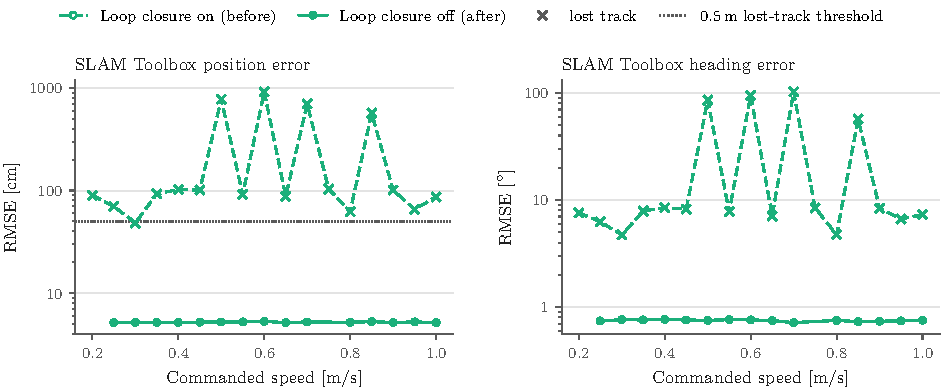
\includegraphics[max width=\linewidth]{figures/slam_before_after.pdf}
  \caption{SLAM Toolbox over speed before (loop closure on, original map \code{victoria\_ref}, dashed)
  and after (loop closure off, loop-closed map \code{victoria\_ref\_lc}, solid). Two runs of the fixed configuration (0.20 and
  \SI{0.75}{m/s}) are missing: their simulation check failed because of a benchmark bug, since
  fixed.}
  \label{fig:slam-ba}
\end{figure}

\begin{table}[htbp]
  \centering\small
  \caption{SLAM Toolbox before and after the fix (3 laps per run, 0.20--\SI{1.00}{m/s}).}
  \label{tab:slam}
  \begin{tabular}{lrrrr}
\toprule
Configuration & \makecell[rb]{{RMSE} \\ {[cm]}} & \makecell[rb]{{p95} \\ {[cm]}} & \makecell[rb]{{Heading} \\ {RMSE [$^\circ$]}} & \makecell[rb]{{Lost} \\ {track}} \\
\midrule
\texttt{victoria\_ref}, loop closure on (before) & 92.9 & 180 & 7.9 & 17/17 \\
\texttt{victoria\_ref\_lc}, loop closure off (after) & 5.2 & 8.0 & 0.7 & 0/15 (+2 failed) \\
\bottomrule
\end{tabular}

\end{table}

The full sweep with the fixed configuration confirmed the single-lap result
(\cref{fig:slam-ba,tab:slam}): \SI{\val{slam-fixed-rmse}}{cm} median RMSE, \SI{\val{slam-fixed-p95}}{cm}
p95 and \ang{\val{slam-fixed-yaw}} heading error, flat over speed, with no run losing track. This
sweep ran six SLAM Toolbox instances in parallel and the simulation slowed to between
\val{slam-fixed-rtf-min} and \val{slam-fixed-rtf-max} of real time, which gives the localizer more
computer time than on the car; a single run at full speed gave the same \SI{5}{cm}.

% =====================================================================
\FloatBarrier
\section{Comparison after the fixes}\label{sec:compare}

\begin{figure}[htbp]
  \centering
  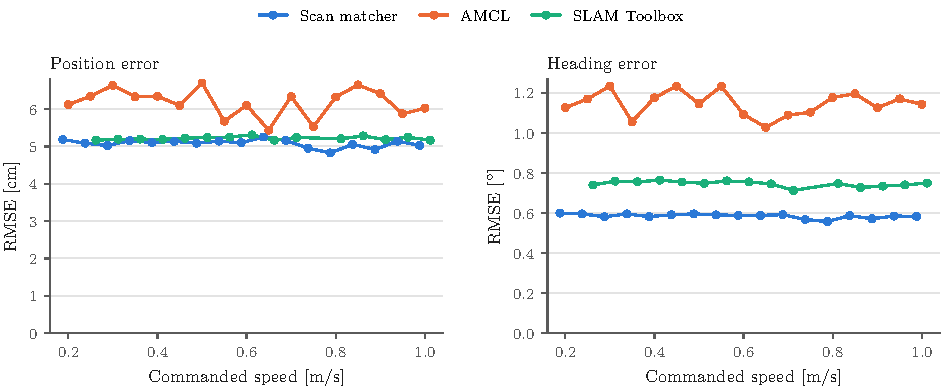
\includegraphics[max width=\linewidth]{figures/final_comparison.pdf}
  \caption{All three localizers after the fixes, perfect odometry, linear scales. Every run kept
  track. The scan matcher ran on the filled map in this sweep.}
  \label{fig:final}
\end{figure}

\begin{table}[htbp]
  \centering\small
  \caption{Perfect odometry after the fixes.}
  \label{tab:final}
  \setlength{\tabcolsep}{4.5pt}
  \begin{tabular}{llrrrrrrr}
\toprule
 & & \multicolumn{4}{c}{Speed sweep, 17 speeds} & \multicolumn{3}{c}{1.0\,m/s, 3 runs${}^{b}$} \\
\cmidrule(lr){3-6}\cmidrule(lr){7-9}
Localizer & Map & \makecell[rb]{{RMSE} \\ {[cm]}} & \makecell[rb]{{p95} \\ {[cm]}} & \makecell[rb]{{Heading} \\ {[$^\circ$]}} & Lost & \makecell[rb]{{RMSE} \\ {[cm]}} & \makecell[rb]{{p95} \\ {[cm]}} & \makecell[rb]{{Heading} \\ {[$^\circ$]}} \\
\midrule
Scan matcher & filled${}^{a}$ & 5.1 & 13.9 & 0.6 & 0/17 & 4.0 & 9.9 & 0.5 \\
AMCL & outline & 6.3 & 11.2 & 1.1 & 0/17 & 6.2 & 11.8 & 1.2 \\
SLAM Toolbox & \texttt{victoria\_ref\_lc} & 5.2 & 8.0 & 0.7 & 0/15 (+2 failed) & 5.2 & 7.9 & 0.8 \\
\bottomrule
\end{tabular}

  \tablenote{${}^{a}$The scan matcher's speed sweep predates the outline map; its 1.0\,m/s
  column is on the outline map. ${}^{b}$Noise level 0 of the noise test: all three on their final
  maps, 3 runs each.}
\end{table}

With both fixes, the three localizers are within \SIrange{4}{6}{cm} of each other
(\cref{fig:final,tab:final}). The scan matcher remains the most accurate in position and heading;
SLAM Toolbox has the smallest bad moments (p95 \SI{8}{cm}); AMCL is about a centimetre behind with
twice the heading error. None depends on speed. As argued in \cref{sec:sweep}, these numbers no
longer separate the localizers in the way that matters on the car.

% =====================================================================
\FloatBarrier
\section{Odometry noise test}\label{sec:noise}

\subsection{Motivation and noise model}

On the car, odometry comes from the motor controller and the IMU through an EKF and drifts; the
localizer's job is to remove that drift. To test this, a node between the simulator and the
localizers corrupts the odometry: each \SI{50}{Hz} step of the car's motion, taken in the car's own
frame, is distorted and integrated from the true start pose (\cref{tab:noise-model}). Level~1 is our
estimate of a real car; level~$k$ multiplies every term by~$k$. The scale errors and the bias always
have the same sign; the random part is seeded, and run~$r$ of every localizer uses seed~$r$, so all
localizers receive the same corrupted odometry. Nothing changes while the car stands still, so the
start pose stays exact. Ground truth is unaffected.

\begin{table}[htbp]
  \centering\small
  \caption{Odometry error model. Level $k$ multiplies every term by $k$.}
  \label{tab:noise-model}
  \begin{tabular}{@{}llp{6.2cm}@{}}
    \toprule
    Error term & Level 1 & Physical counterpart \\
    \midrule
    Distance scale & $+2\,\%$ & motor-controller speed gain or tire radius slightly off \\
    Yaw-rate scale & $+2\,\%$ & steering or gyroscope scale error \\
    Gyroscope bias & \SI{0.2}{\degree/s} & heading creeps even on a straight \\
    Random walk, position & \SI{1}{cm}\,/\,$\sqrt{\mathrm{m}}$ & per-step noise along and across \\
    Random walk, heading & \ang{0.3}\,/\,$\sqrt{\mathrm{m}}$ & per-step heading noise \\
    \bottomrule
  \end{tabular}
\end{table}

\begin{figure}[htbp]
  \centering
  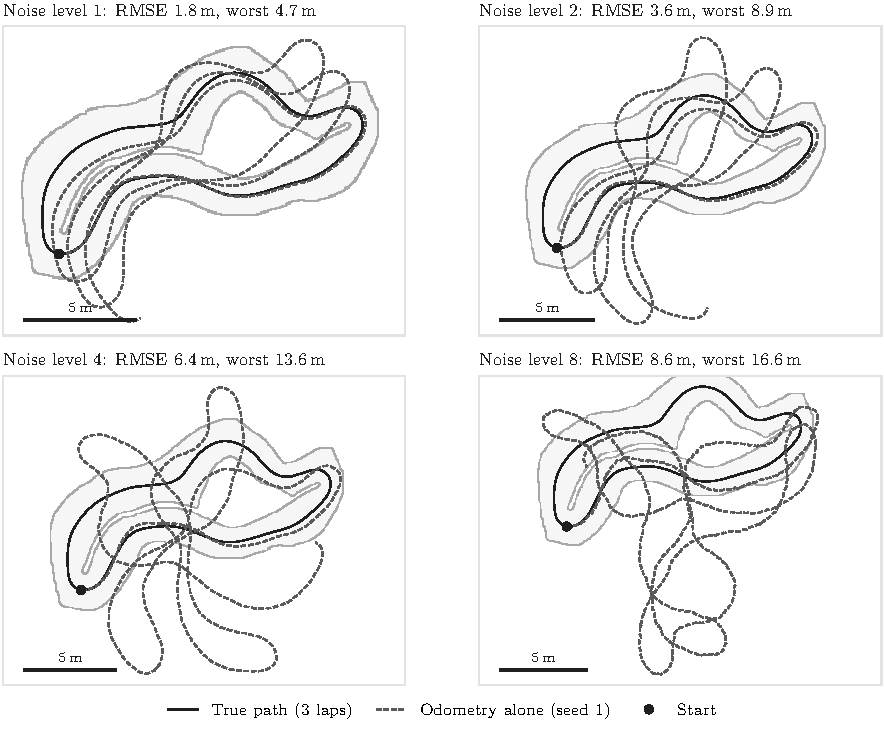
\includegraphics[max width=\linewidth]{figures/odom_drift.pdf}
  \caption{What the localizers have to correct: the odometry alone (no localizer, seed 1) over three
  laps at each noise level, against the true path. At level 1 the odometry is about \SI{1.5}{m}
  and \ang{10}--\ang{13} off after one lap.}
  \label{fig:odom-drift}
\end{figure}

\Cref{fig:odom-drift} shows the effect: already at level~1, the odometry alone ends the first lap
more than a metre from the truth, and over three laps it wanders several metres away. The level-1
values are an estimate, not a measurement from our car.

\subsection{Test design}

\begin{table}[htbp]
  \centering\small
  \caption{Noise-test matrix.}
  \label{tab:noise-design}
  \begin{tabular}{@{}ll@{}}
    \toprule
    Parameter & Value \\
    \midrule
    Localizers & scan matcher, AMCL, SLAM Toolbox (final configurations) and odometry only \\
    Noise levels & 0 (perfect), 1, 2, 4, 8 \\
    Runs per level & 3 (seeds 1--3, the same seeds for every localizer) \\
    Speed and laps & \SI{1.0}{m/s}, 3 laps per run \\
    Total & \val{runs-noise} runs on 5 parallel workers (about \SI{30}{min}) \\
    Real-time factor & \val{noise-rtf-min}--\val{noise-rtf-max} \\
    \bottomrule
  \end{tabular}
\end{table}

\Cref{tab:noise-design} lists the matrix. Speed was fixed at \SI{1.0}{m/s} because the sweep had
shown no speed dependence, and three seeds per level replace the one-run-per-speed design, since
here the random part of the noise differs between runs. The \emph{odometry only} case runs no
localizer at all (a fixed identity \code{map}$\to$\code{odom}); its error is the drift a localizer
has to remove. With five instead of six workers the simulation stayed close to real time.

\subsection{Results}

\begin{figure}[htbp]
  \centering
  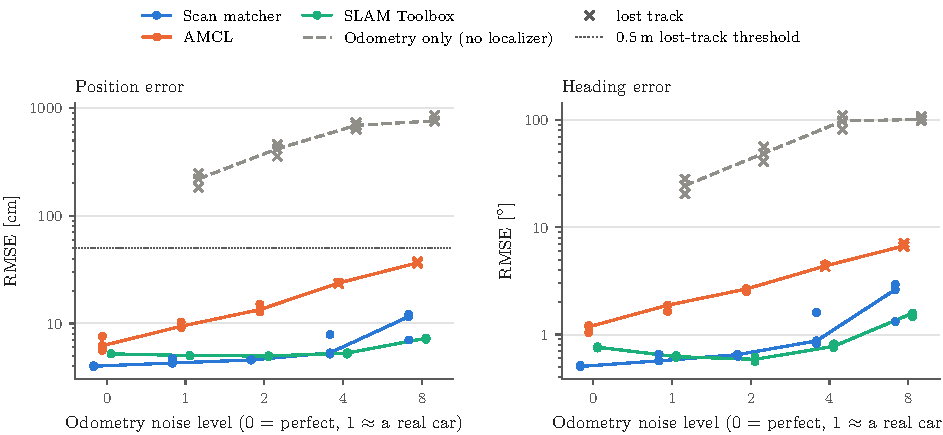
\includegraphics[max width=\linewidth]{figures/noise_rmse.pdf}
  \caption{Position and heading RMSE over odometry noise level (log scales); one dot per run, lines
  through the medians. The dashed grey line is the odometry alone (zero at level 0, so not drawn
  there). SLAM Toolbox stays nearly flat; the scan matcher degrades at level 8; AMCL's error grows
  steadily and it loses track at levels 4 and 8.}
  \label{fig:noise-rmse}
\end{figure}

\begin{table}[htbp]
  \centering\small
  \setlength{\tabcolsep}{3.6pt}
  \caption{Noise test: medians over three runs per level. RMSE and p95 in cm, heading (Hdg) RMSE in
  degrees, lost = runs that exceeded \SI{0.5}{m}.}
  \label{tab:noise}
  \begin{tabular}{crrrrrrrrrrrrr}
\toprule
 & \multicolumn{4}{c}{Scan matcher} & \multicolumn{4}{c}{AMCL} & \multicolumn{4}{c}{SLAM Toolbox} & Odom. only \\
\cmidrule(lr){2-5}\cmidrule(lr){6-9}\cmidrule(lr){10-13}\cmidrule(lr){14-14}
Level & RMSE & p95 & Hdg & Lost & RMSE & p95 & Hdg & Lost & RMSE & p95 & Hdg & Lost & RMSE [m] \\
\midrule
0 & 4.0 & 9.9 & 0.5 & 0/3 & 6.2 & 11.8 & 1.2 & 0/3 & 5.2 & 7.9 & 0.8 & 0/3 & 0 \\
1 & 4.3 & 10.6 & 0.6 & 0/3 & 9.4 & 16.1 & 1.9 & 0/3 & 5.0 & 7.9 & 0.6 & 0/3 & 2.20 \\
2 & 4.6 & 10.9 & 0.6 & 0/3 & 13.4 & 23.3 & 2.7 & 0/3 & 5.0 & 7.8 & 0.6 & 0/3 & 4.19 \\
4 & 5.3 & 11.8 & 0.9 & 0/3 & 23.7 & 36.7 & 4.4 & 1/3 & 5.3 & 8.4 & 0.8 & 0/3 & 6.90 \\
8 & 11.6 & 20.4 & 2.6 & 0/3 & 36.5 & 61.4 & 6.7 & 3/3 & 7.3 & 12.3 & 1.6 & 0/3 & 7.62 \\
\bottomrule
\end{tabular}

\end{table}

\Cref{fig:noise-rmse,tab:noise} summarize the results; \cref{fig:noise-lap} shows where along the
laps the errors occur at the two highest levels.
\begin{itemize}[leftmargin=1.5em]
  \item \swatch{slam}~\textbf{SLAM Toolbox} was the most robust: \SI{\val{slam-n0-rmse}}{cm} with
        perfect odometry, \SI{\val{slam-n4-rmse}}{cm} at level 4 and \SI{\val{slam-n8-rmse}}{cm} at
        level 8, never lost, with the smallest spread between seeds.
  \item \swatch{scan}~\textbf{The scan matcher} was the most accurate up to level 2 and level with
        SLAM Toolbox at level 4 (\SI{\val{scan-n0-rmse}}{cm} to \SI{\val{scan-n4-rmse}}{cm}), but
        roughly doubled its error at level 8 (\SI{\val{scan-n8-rmse}}{cm}, heading
        \ang{\val{scan-n8-yaw}}). It never lost track.
  \item \swatch{amcl}~\textbf{AMCL}'s error grew with every level, from \SI{\val{amcl-n0-rmse}}{cm}
        to \SI{\val{amcl-n4-rmse}}{cm} at level 4 and \SI{\val{amcl-n8-rmse}}{cm} at level 8. It lost
        track in \val{amcl-n4-lost} runs at level 4 and \val{amcl-n8-lost} at level 8, but without the
        multi-metre jumps of the filled map: its worst errors were 0.4--\SI{1.0}{m}.
  \item \swatch{odom}~\textbf{The odometry alone} was off by \SI{\val{odom-n1-rmse}}{m} RMSE at
        level 1 and \SI{\val{odom-n8-rmse}}{m} at level 8; all three localizers removed most of it.
\end{itemize}

\begin{figure}[htbp]
  \centering
  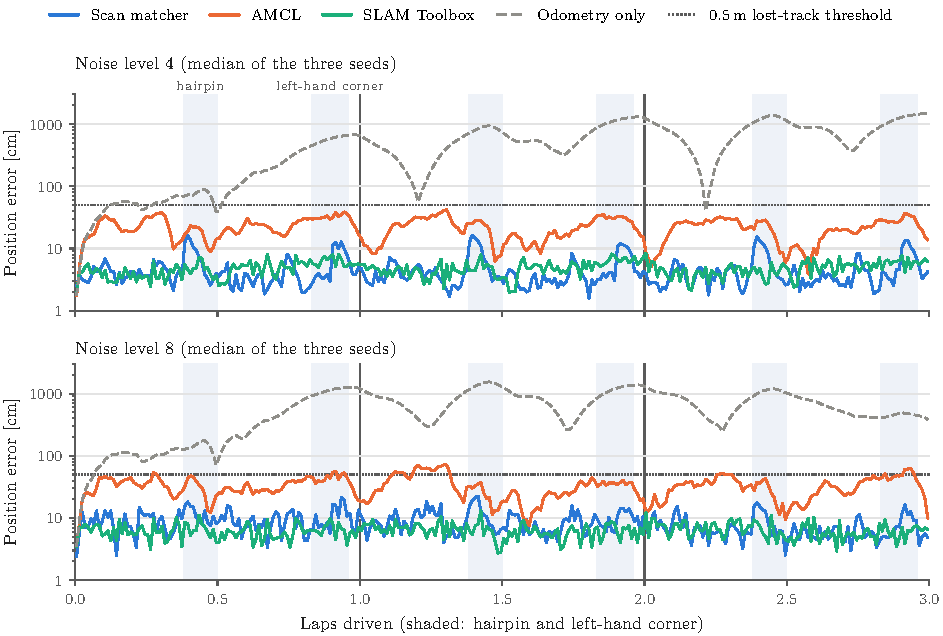
\includegraphics[max width=\linewidth]{figures/noise_along_lap.pdf}
  \caption{Position error along the three laps at noise levels 4 and 8 (median of the three seeds,
  log scale; shaded: hairpin and left-hand corner). AMCL's error follows the odometry's pattern at
  a fraction of its size and touches the lost-track threshold at level 8; the scan matcher and SLAM
  Toolbox stay around \SIrange{3}{15}{cm}, with the scan matcher's peaks in the corners.}
  \label{fig:noise-lap}
\end{figure}

These differences are consistent with how the methods work, although we have not tested the
explanations separately. AMCL spreads its particles by a fixed fraction of each odometry step and
corrects them with flat likelihood-field weights, so a systematic odometry error is only partly
removed before the next step adds more. The scan matcher refines each scan from the odometry
prediction with a local Gauss--Newton fit, which works well until the odometry error between scans
grows large. SLAM Toolbox first searches a grid of poses around the prediction (correlative
matching) before refining, which tolerates larger errors per step.

% =====================================================================
\FloatBarrier
\section{Conclusions}\label{sec:conclusions}

\begin{itemize}[leftmargin=1.5em]
  \item The speed sweep showed no speed dependence for any localizer between 0.20 and
        \SI{1.00}{m/s}. Its value lay in locating the failures, which led to two configuration
        problems rather than algorithmic limits.
  \item AMCL must be given a walls-only map. On the race stack's filled map, beams that overshoot a
        wall count as hits, the particle weights flatten, and the estimate jumps; on the outline map
        its error halved (\SI{\val{amcl-sweep-rmse}}{cm} to \SI{\val{amcl-outline-rmse}}{cm}) and it
        no longer lost track.
  \item SLAM Toolbox must run with loop closure off in localization mode, on a map recorded with
        loop closure. Loop closure in localization re-optimizes the whole graph and moves the map on
        wrong matches; without it the map stays fixed and the error fell from
        \SI{\val{slam-sweep-rmse}}{cm} to \SI{\val{slam-fixed-rmse}}{cm}.
  \item With perfect odometry, all three reach \SIrange{4}{6}{cm}, a level that measures disturbance
        rather than correction.
  \item Under odometry noise the ranking becomes clear: SLAM Toolbox is the most robust
        (\SI{\val{slam-n8-rmse}}{cm} at eight times our real-car estimate), the scan matcher is the most
        accurate at low noise and level with SLAM Toolbox at four times that estimate, and AMCL
        degrades steadily and loses track at the highest levels.
\end{itemize}

\begin{thebibliography}{9}\small
\bibitem{macenski2021slam}
S.~Macenski and I.~Jambrecic, ``SLAM Toolbox: SLAM for the dynamic world,'' \emph{Journal of Open
Source Software}, vol.~6, no.~61, p.~2783, 2021.
\bibitem{macenski2020marathon}
S.~Macenski, F.~Mart\'in, R.~White, and J.~Gin\'es Clavero, ``The Marathon 2: A navigation
system,'' in \emph{Proc.\ IEEE/RSJ Int.\ Conf.\ Intelligent Robots and Systems (IROS)}, 2020.
\bibitem{thrun2005probabilistic}
S.~Thrun, W.~Burgard, and D.~Fox, \emph{Probabilistic Robotics}. MIT Press, 2005.
\bibitem{fox2003kld}
D.~Fox, ``Adapting the sample size in particle filters through KLD-sampling,'' \emph{The
International Journal of Robotics Research}, vol.~22, no.~12, pp.~985--1003, 2003.
\end{thebibliography}

\end{document}
